%!TEX TS-program = pdflatex
%!TEX encoding = UTF-8 Unicode
\documentclass[11pt,a4paper]{article}

\usepackage[T1]{fontenc}
\usepackage[utf8]{inputenc}
\usepackage[margin=1.15cm]{geometry}
\usepackage{enumitem}
\usepackage{titlesec}
\usepackage[hidelinks]{hyperref}
\usepackage{graphicx}
\usepackage{xcolor}
\usepackage{tabularx}

\setlength{\parindent}{0pt}
\setlength{\parskip}{2.5pt}
\setlist[itemize]{leftmargin=1.2em, itemsep=1pt, topsep=1pt, parsep=0pt}

\pagenumbering{gobble}

\titleformat{\section}
  {\large\bfseries}
  {}
  {0pt}
  {}
  [\vspace{2pt}\color{black!40}\rule{\textwidth}{0.4pt}]
\titlespacing*{\section}{0pt}{6pt}{3pt}

\newcommand{\resumeEntry}[4]{
\begin{tabularx}{\textwidth}{@{}Xr@{}}
\textbf{#1} & #2 \\
\textit{#3} & \textit{#4} \\
\end{tabularx}
\vspace{-3pt}
}

\begin{document}

% ===== HEADER =====
\begin{minipage}[c]{0.80\textwidth}
{\LARGE \textbf{Mohammed EZ-ZOUAK}}\\
\textbf{Junior Full-Stack Developer}\\[3pt]
Casablanca, Morocco \textbar\ (+212) 06-0203-7451 \textbar\ \href{mailto:m.ezzouak@outlook.com}{m.ezzouak@outlook.com}\\
\href{https://linkedin.com/in/mohammed-ez-zouak}{linkedin.com/in/mohammed-ez-zouak} \textbar\ \href{https://github.com/mezzouak}{github.com/mezzouak} \textbar\ \href{https://mezzouak.tech}{mezzouak.tech}
\end{minipage}
\hfill
\begin{minipage}[c]{0.17\textwidth}
\raggedleft
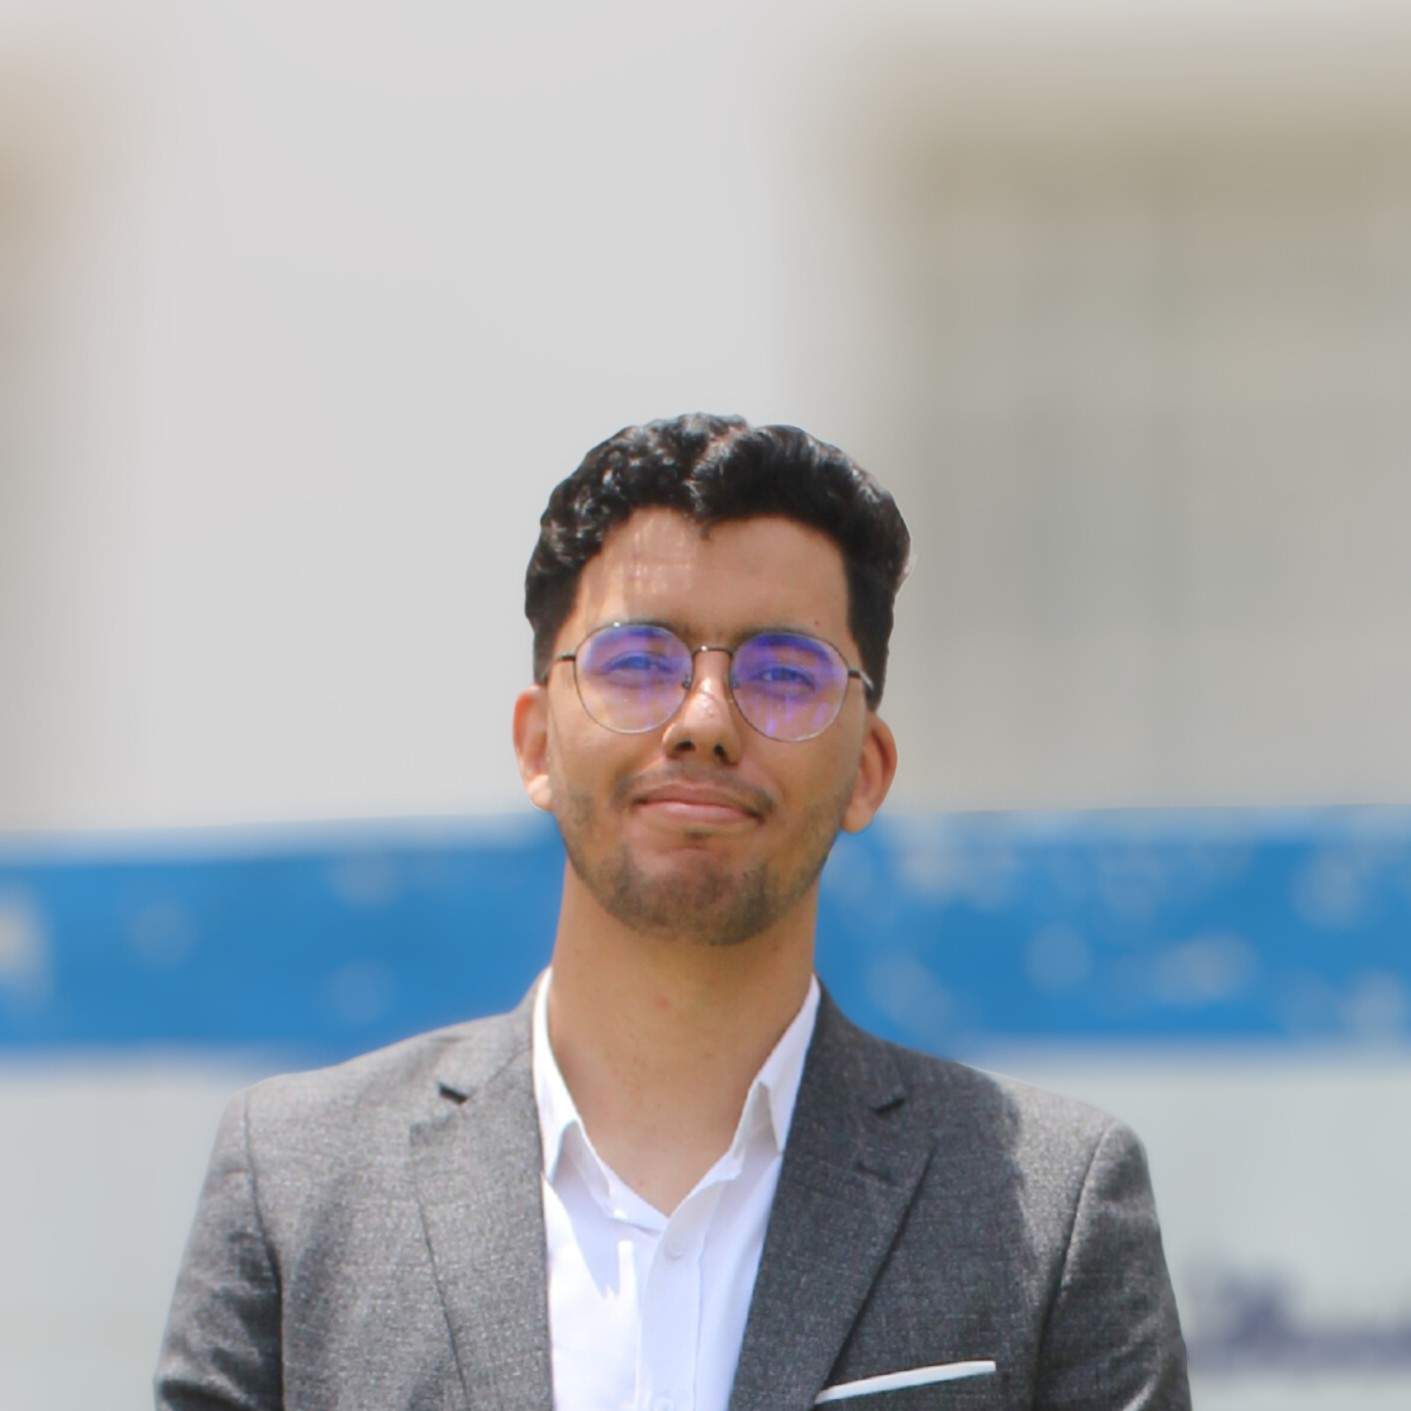
\includegraphics[width=0.9\linewidth]{profile_pic.jpg}
\end{minipage}

\vspace{2pt}

% ===== SUMMARY =====
\section*{Summary}
Junior Full-Stack Developer with hands-on experience building and deploying web applications using Python (Django). Contributed to production systems serving thousands of daily users, with a focus on backend development, database performance, and real-time features.

% ===== EXPERIENCE =====
\section*{Experience}

\resumeEntry
{Software Engineer (Junior)}
{2025-08 -- Present}
{ITSS Paris}
{Casablanca, Morocco}

\begin{itemize}
  \item Contributed to backend development of Django-based platforms, including IJConnect (\textasciitilde5K daily users).
  \item Improved performance of database-heavy pages by identifying bottlenecks (AWS RDS insights) and applying indexing and query optimizations, reducing load times from several minutes to \textasciitilde30 seconds.
  \item Implemented real-time notifications using WebSockets and integrated chat via a Matrix server.
  \item Participated in client communication, requirement estimation (chiffrage), development, and deployment.
  \item Worked across multiple client projects in a multi-tenant environment.
\end{itemize}

\resumeEntry
{Software Engineer Intern}
{2025-02 -- 2025-07}
{Lear Corporation}
{Kenitra, Morocco}

\begin{itemize}
  \item Developed a proof-of-concept defect detection system using YOLO and OpenCV (\textasciitilde77\% precision / 75\% recall).
  \item Built dashboards to visualize production KPIs (defect rate, throughput, downtime).
  \item Contributed to MVP tools supporting digitalization of internal workflows.
\end{itemize}

\resumeEntry
{Freelance / Contract Developer}
{2025-01 -- 2025-02}
{Twins Groupe}
{Fes, Morocco}

\begin{itemize}
  \item Implemented a search feature using Apache Solr in a Drupal-based platform.
  \item Supported backend development and templating tasks during a short-term engagement.
\end{itemize}

% ===== EDUCATION =====
\section*{Education}

\resumeEntry
{State Engineering Degree in Computer Science -- Specialization: Information Systems and Decision Support}
{2020 -- 2025}
{ENSA Tetouan}
{Tetouan, Morocco}

% ===== SKILLS =====
\section*{Technical Skills}

\textbf{Backend \& APIs:} Python (Django), REST APIs, WebSockets \\
\textbf{Databases:} PostgreSQL, MySQL, query optimization, indexing \\
\textbf{Data Engineering \& AI:} Airflow, dbt, GCP, YOLO, OpenCV \\
\textbf{Web:} JavaScript, React (basic), HTML, CSS \\
\textbf{Cloud \& Tools:} Google Cloud Platform, Docker, Git

% ===== LANGUAGES =====
\section*{Languages}

Arabic (Native) \quad French (C1) \quad English (C1)

\end{document}